% !TEX root =../pfcTipoETSI.tex
%El anterior comando permite compilar este documento llamando al documento raíz
\chapter{Introducción}\LABCHAP{intro}
%\epigraph{}{}

%\lettrine[lraise=0.7, lines=1, loversize=-0.25]{E}{n}
\lettrine[lraise=-0.1, lines=2, loversize=0.2]{P}{r}oducir burbujas de tamaño micrométrico tiene, hoy día, numerosas aplicaciones que van más allá de aquellas destinadas a procesos  a escala de laboratorio. De hecho, el gran desarrollo y la diversidad de tecnologías desarrolladas en los últimos años han dado lugar a recientes revisiones del estado del arte que tratan con gran detalle tanto los fundamentos que sustentan la producción de microburbujas monodispersas como sus aplicaciones (véase~\cite{Rodriguez-Rodriguez2015b}). Tanto es así que el empleo de microburbujas tiene cabida en procesos de índole tan variada como el tratamiento de aguas, la industria alimentaria, y todo tipo de procesos médicos y farmacológicos, por citar algunos ejemplos. Así, para la obtención de imágenes por ultrasonidos, el uso de microburbujas como angentes de contraste ha demostrado arrojar unos excelentes resultados \cite{Ferrara2007,Kilbanov2006,Postema2005}. Por otro lado, las elevadas necesidades de aireación y el gran porcentaje que esta ocupa en el coste de operación de los biorreactores~\cite{Garcia-Ochoa2009,Rosso2008} hacen que el adecuado control del tamaño y la frecuencia de producción de las burbujas tenga un fuerte impacto en la eficiencia del proceso. 


Cuando se requiere el uso de microburbujas en aplicaciones como las mencionadas anteriormente, se dispone de tres variables que se desean controlar: el diámetro medio de las burbujas, $d_{b}$, la frecuencia de producción de estas, $f_{b}$ y el índice de polidispersión, PDI, ya que para considerar que la producción de microburbujas es monodispera estas tienen que tener un PDI por debajo del 5\%~\cite{Rodriguez-Rodriguez2015b}. Así, en el caso de la oxigenación de biorreactores, típicamente será necesario satisfacer la demanda de oxígeno de los microorganismos presentes, OUR~(\emph{Oxygen Uptake Rate}, de sus siglas en inglés), por lo que el ratio de transferencia de oxígeno~(\emph{Oxygen Transfer Rate}-OTR) puede ser el paso limitante en todo el proceso~\cite{Garcia-Ochoa2009}. El parámetro que controla el OTR es, dado un gradiente de concentración, el coeficiente de transferencia de masa, $k_{L}a$, el cual se encuentra direcamente afectado por la frecuencia y el diámetro de las burbujas. En efecto, el area específica de interfase, i.e. el area por unidad de volumen de las burbujas, depende de forma inversa del diámetro de las burbujas ($a = 6\phi/d_{b}$, con $\phi$ la fracción de gas en el medio). Por lo tanto, a menor diámetro de las burbujas mayor es el coeficiente de transferencia de transferencia de masa, lo que se traduce en última instancia en una reducción del caudal de aire requerido para satisfacer el OUR del cultivo, con el consiguiente ahorro que esta implica. Es por ello que el empleo de difusores de burbuja fina \cite{Sander2017,Rosso2008}, con diámetros 1-3~mm, o incluso de microburbujas \cite{Terasaka2011,Kawahara2009,Sadatomi2005}, con diámetros 10-500~$\mu$m, resulta esencial cuando se trata de aumentar la eficiencia del proceso de aireación; no obstante, también se ha reportado que la presencia de surfactantes y antiespumantes en el medio puede reducir críticamente el valor de dicho coeficiente en los casos en los que se favorece la coalescencia (véase~\cite{Garcia-Ochoa2005}), mientras que la presencia de una determinada concentración de sal (equivalente al lodo presente en las aguas no tratadas) puede inhibir precisamente esta coalescencia~\cite{Sander2017}. 

Como puede observarse, las exigencias de las industrias actuales, que requieren cada vez mayores frecuencias de producción y menores diámetros de las burbujas, conlleva que se hayan desarrollado diferentes tecnologías para poder conseguir una población monodispersa donde se pueda controlar tanto $d_{b}$ y $f_{b}$. Todas estas tecnologías emergentes emplean dispositivos microfluídicos de tamaño milimétrico y submilimétrico que, aunque puedan parecer muy similares entre sí, se fundamentan en principios físicos diferentes que conviene comprender~\cite{Rodriguez-Rodriguez2015b}. De este modo, el capítulo se estructura de la siguiente forma: en primer lugar, se realiza una descripción de las ecuaciones que gobiernan la dinámica de una burbuja que se produce en el seno de un líquido, después, se enumeran las diversas tecnologías que se han desarrollado y que se utilizan para generar una población monodispersa de microburbujas en los diferentes regímenes. En algunas de esta aplicaciones, el papel del gradiente de presión existente en el líquido exterior juega un papel fundamental que se describe con detalle en la \SEC{gradPres}. Finalmente, considerando las pequeñas geometrías empleadas en las tecnologías actuales y el rol determinante del gradiente de presión, se expondrán las ideas que han llevado al desarrollo del dispositivo que en este trabajo se estudia. 

\section{Fundamentos de la generación de burbujas}\LABSEC{fundamentos}

Lejos de lo que pudiera intuirse, la generación de burbujas es un proceso con importantes diferencias respecto al procceso de producción de gotas. En general, para generar gotas de radio $r_{d}$ a una frecuencia $f_{d}\sim U/r_{d}$, basta con injectar el líquido a través de un tubo de radio $r_{t}\sim r_{d}$ a una velocidad $U \gtrsim U_{c}$, con $U_{c} = \left[\sigma/\left(\rho g\right)\right]^{1/2}$ la velocidad capilar\footnote{Se remite al lector interesado en la rotura e inestabilidades de chorros líquidos a la excelente revisión~\cite{Eggers2008}}~\cite{Rodriguez-Rodriguez2015b}. 

Sin embargo, en el caso de la formación  de burbujas para estas condiciones, el comportamiento es diferente. Por un lado, en el caso de generación cuasiestática en el que $U \ll U_{c}$, el radio de la burbuja viene dado por el conocido \emph{radio de Fritz}, que resulta del balance de esfuerzos de tensión superficial con la fuerza de flotación, $r_{F}/r_{t} \sim \left[3/(2Bo)\right]^{1/3}$, con $Bo = \rho g r_{t}^{2}/\sigma$ el número de Bond, que mide la importancia relativa de los esfuerzos de tensión superficial frente a los esfuerzos de volumen  (gravedad/flotación). Sin embargo, si se desea reducir el diámetro de las burbujas o incrementar la frecuencia de producción aumentando la velocidad de inyección del gas a valores por encima de $U_{c}$, lejos de obtener un chorro de radio comparable al del injector, se obtienen (por encima de cierta velocidad) burbujas de volumen $V_{b} \propto \left(Q_{g}/g^{1/2}\right)^{6/5} > 4/3\pi r_{F}^{3}$~\cite{Rodriguez-Rodriguez2015b}, y lo que es más, si se sigue aumentando la velocidad, las burbujas cercanas entresí pueden coalescer, con lo que el diámetro final obtenido es mucho mayor~\cite{Higuera2006}. 

Para explicar estas diferencias entre ambos procesos, si se desprecian los efectos dinámicos del gas (ya que $\rho_{g}/\rho \gg 1$ y $\mu_{g}/\mu  \gg 1$), y se considera que la burbuja es prácticamente esférica, con una presión uniforme en su interior, la dinámica de la burbuja puede describirse a través de la ecuación de Rayleigh-Plesset.

\begin{equation}\LABEQ{rayleighPlesset}
\rho\left(R_{b}\ddot{R}_{b} + \dfrac{3}{2}\dot{R}_{b}^{2}\right) = \Delta p_{exit} - \dfrac{2\sigma}{R_{b}} - 4\mu \dfrac{\dot{R}_{b}}{R_{b}}
\end{equation}

Tal y como se puede observar en~\cite{Rodriguez-Rordiguez2015b}, para que el crecimiento de la burbuja y su posterior colapso tengan lugar, requiere que el término $\Delta p - 2\sigma/R_{b}$ cambie de positivo, valor que adquire en los primeros instantes mientras la burbuja se infla, a negativo, momento en el que las velocidades negativas cerca del inyector  la harán colapsar. La \EQ{rayleighPlesset} junto con la ecuación de continuidad

\begin{equation}\LABEQ{continuidad}
Q_{g} = \dfrac{\mathrm{d}V_{b}}{\mathrm{d}t} \simeq 4\pi R_{b}^{2} \dot{R}_{b}
\end{equation}

y el balance de cantidad de movimiento en la línea de gas\footnote{Nótese que no puede presuponerse, \textit{a priori}, la constancia del caudal, debido a las dos etapas bien diferenciadas que existen en el proceso de generación de burbujas.}

\begin{equation}\LABEQ{continuidad}
p_{0} - p_{exit} = \rho_{g}K\left(Re_{g}\right)\left[Q_{g}/\left(\pi r_{t}^{2}\right)\right]^{2}
\end{equation}

proporcionan el conjunto de ecuaciones necesario para describir sucintamente las tecnologías de la \SEC{tecnologias} y, con ellas, el diámetro y frecuencia de producción de las burbujas finalmente obtenidas. 
\begin{figure}[hbtp!]
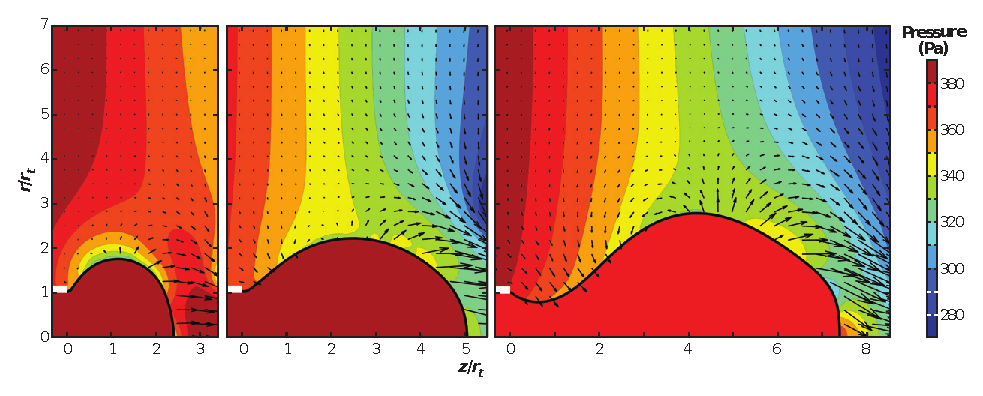
\includegraphics[width=\linewidth]{introduccion/figuras/esquemaBurbuja.eps}
\caption{Contornos de presión en las fases iniciales del proceso de formación de una burbuja para un número de Bond, $Bo = 0.245$. Cortesía de~\cite{Rodriguez-Rodriguez2015b}}
\LABFIG{esquemaBurbuja}
\end{figure}

Sintetizando una vez más las ideas expuestas en~\cite{Rodriguez-Rodriguez2015b}, el proceso de formación de una burbuja en una piscina en reposo puede esquematizarse en las siguientes etapas:

\begin{itemize}
\item En primer lugar, para satisfacer \EQ{continuidad}, el volumen de la burbuja debe aumentar, lo que provoca velocidades radiales en el líquido hacia fuera de la burbuja. 
\item La presión del gas en el interior de la burbuja es prácticamente uniforme, y debe adaptarse a la del líquido exterior en algún punto entre $z = 0$ (véase la \FIG{esquemaBurbuja}) y $z = 2R_{b}$, el cenit de la misma, supóngase en $z \sim R_{b}$. 
\item A medida que el radio de la burbuja aumenta, la punta de la burbuja se encuentra con una sobrepresión respecto al líquido exterior del orden de $\sim \rho g R_{b}$, lo que contribuye a que el gas acelere al líquido exterior, mientras que, en $z = 0$, es el líquido el que ejerce una sobrepresión sobre la base de la burbuja del orden de $\sim -\rho g R_{b}$, lo que conlleva que el líquido induzca velocidades hacia el interior de la burbuja. 
\end{itemize}

Por lo tanto, si nos ceñimos al caso no viscoso, la burbuja se desprenderá del inyector cuando la velocidad hacia adentro en $z = 0$, que surge del balance de \EQ{rayleighPlesset}, $\Delta p = p_{exit} - 2\sigma/R_{b} \sim \rho \dot{R}_{b}$ coincida con la velocidad hacia afuera impuesta por continuidad, $\sim Q_{g}/\left(4\pi R_{b}^{2}\right)$.

\begin{equation}\LABEQ{dbestimado}
\dfrac{Q_{g}}{R_{b}^{2}} \sim 	\sqrt{\dfrac{\Delta p}{\rho}} \sim \sqrt{g R_{b}} \Rightarrow d_{b} \sim \left(\dfrac{Q_{g}}{g^{1/2}}\right)^{2/5}
\end{equation}

siendo, finalmente, la frecuencia de producción 

\begin{equation}\LABEQ{fbestimado}
f_{b}\sim \dfrac{Q_{g}}{d_{b}^{3}} \sim	\left(\dfrac{g^{3}}{Q_{g}}\right)^{1/5}
\end{equation}

Así, aunque puede emplearse este sencillo método para producir burbujas simplemente inyectando gas en el seno de un líquido en reposo, la burbujas obtenidas poseen un diámetro significativamente mayor que el radio del inyector y con frecuencias que decrecen con el caudal, por lo que no resulta un método adecuado para satisfacer las demandas que las aplicaciones actuales requieren en lo que a diámetros y frecuencias se refiere\cite{Rodriguez-Rodriguez2015b}. Ello ha propiciado el desarrollo de tecnologías más sofisticadas basadas en dispositivos microfluídicos los cuales, en esencia, buscan aumentar el gradiente de presión (esto es, la gravedad efectiva) al que se ve sometida la gota en su proceso de generación. 




\section{Dispositivos para la generación de microburbujas}\LABSEC{tecnologias}


Una vez que se han descrito las ecuaciones necesarias para la compresión de los fundamentos de la generación de burbujas en el seno de un líquido, se está en disposición de enumerar y describir de forma sucinta las tecnologías más relevantes que, actualmente, se emplean para producir masivamente las mencionadas burbujas. Conviene recordar que las soluciones tecnológicas que aquí se presentan no son las únicas que permiten la producción de burbujas con tamaños submilimétricos; en efecto, en aplicaciones industriales como los reactores químicos, los esfuerzos de cortadura fruto de la turbulencia son los responsables de que la formación de burbujas que, aunque micrométricas y a grandes frecuencias, son generadas con un alto PDI~\cite{Rodriguez-Rodriguez2015b}.

De nuevo, al igual que se realizó en \SEC{fundamentos}, se respetará la estructura de~\cite{Rodriguez-Rodriguez2015b} para presentar las tecnologías que a continuación se describen, no extendiénsose en exceso y pudiendo encontrar el lector una descripción más detallada tanto en el \textit{review} como en las referencias citadas en él. Así pues, en la \FIG{tecnologias}, se describen de forma esquemática los dispositivos más relevantes para la producción de burbujas actualmente. En la figura se pueden distinguir dos tipos principales de tecnologías: aquellas emplean una corriente de líquido para provocar el colapso de la corriente gaseosa para la formación de burbujas (\FIG{tecnologias}a-d) y aquellas que en las que se emplean ultrasonidos (\FIG{tecnologias}e-f). A su vez, de entre las primeras, se puede distinguir en aquellas en las que el líquido es inyectado en la misma dirección que la corriente gaseosa (\FIG{tecnologias}a-c) y aquellas en las que el líquido y el gas se encuentran de forma perpendicular (\FIG{tecnologias}d). Finalmente, la diferencia principal entre los dispositivos de \emph{flow-focussing} (\FIG{tecnologias}b-c), y los de \emph{coflow} es que en el primero se hace pasar ambos fluidos a través de un estrechamiento, lo que acelera colapso y permite generar burbujas más pequeñas~\cite{Rodriguez-Rodriguez2015b}. En esta sección, nos centraremos sólo en los 4 primeros, debido a la analogía que los mismos presentan con la solución tecnológica de la que trata este estudio. 


\begin{figure}
\LABFIG{tecnologias}
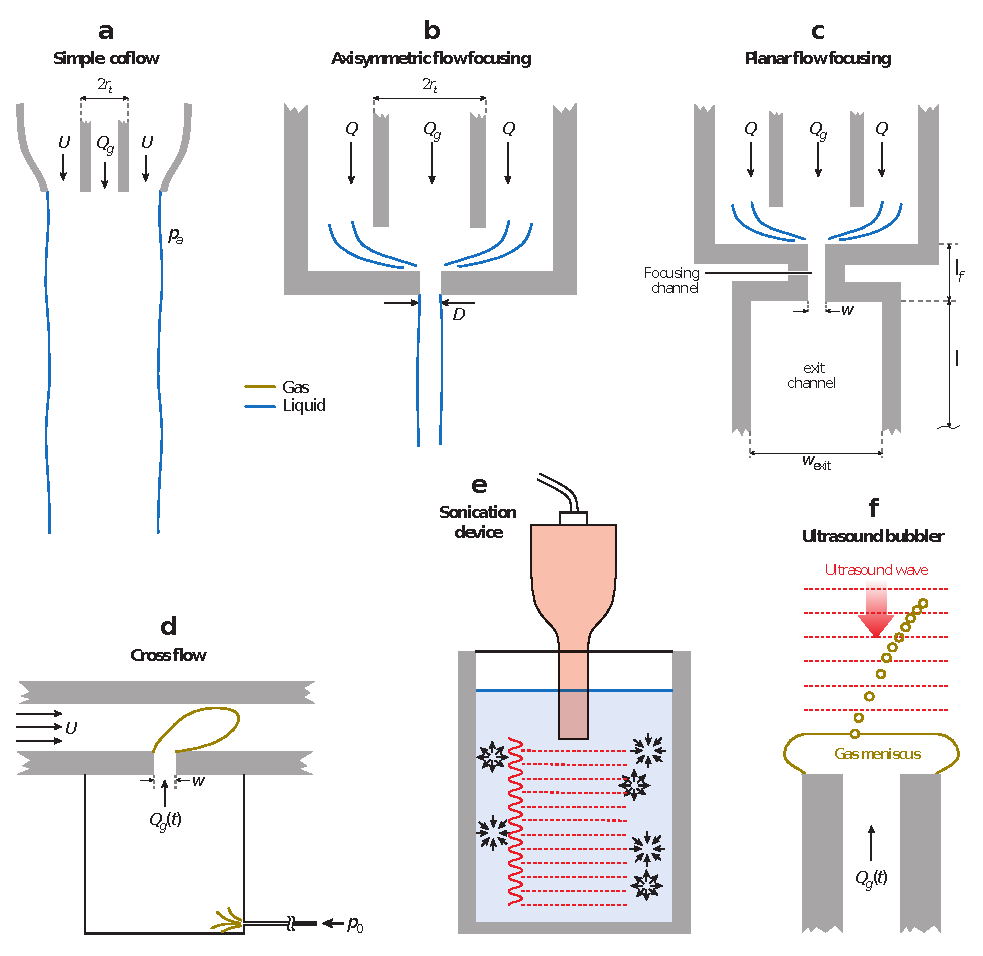
\includegraphics[scale=1]{introduccion/figuras/tecnologias.eps}
\caption{Representación esquemática de los diferentes dispositivos que identiican la tecnología utilizada en la producción de burbujas monodispersas. Figura adaptada de~\cite{Rodriguez-Rodriguez2015b}.}
\LABFIG{tecnologias}
\end{figure}

\subsection{Dispositivos de Coflow}\LABSSEC{coflow}

Un dispositivo de tipo coflow es aquél como el mostrado en la \FIG{tecnologias}a, donde la corriente gaseosa y la de líquido son inyectadas en la misma dirección y de forma libre. Las condiciones en las que usualmente se opera este tipo de dispositivos son aquellas en las que el número de Reynolds y Webber son tales que $Re = \rho U r_{t}/\mu \gg 1$ y $We = \rho U^{2} r_{t}/ \sigma$. Bajo estas condiciones, las frecuencias de producción, $f_{b}$ y los diámetros equivalentes de las burbujas obtenidas, $d_{b} = \left[\left(6Q_{g}\right)/\left(\pi f_{b}\right)\right]^{\left(1/3\right)} $, dependen sólo del ratio de velocidades gas-líquido, $U_{g}/U$, y del ratio $r_{t}/U$. Además, en los casos bajo consideración donde $We \gg 1$, el líquido exterior impone la velocidad a la que la interfase es transportada, con lo que se previene la coalescencia ya que las burbujas son transportadas a la velocidad del líquido~\cite{Sevilla2005a}. Precisamente, en una operación normal con este tipo de dispositivos, la velocidad del gas suele ser mayor que la del líquido, con lo que las burbujas son generadas cerca de la punta del inyector. Siguiendo las mismas ideas que el proceso basado en las fases de expansión y posterior colapso descrito en \SEC{fundamentos}, en \cite{Gordillo2007a} se desarrolla un modelo simple para la fase de colapso en el que puede comprobarse que, en el límite en el que $U_{g}/U \gg 1$, la frecuencia escala como $f_{b}\simeq 0.15U/r_{t}$. 

Por otro lado, el caso contrario en el que $Re \ll 1$ no ha sido muy reportado en la literatura~\cite{Rodriguez-Rodriguez2015b}. En este caso, en lugar del número de Webber, el parámetro adimensional que gobierna el problema es el número capilar, $Ca = \mu U /\sigma$, además del ratio $U_{g}/U$ como en el caso anterior y del ya descrito número de Bond, $Bo$. En este caso, tras el exhaustivo estudio numérico de~\cite{Suryo2006a}, se tiene que el diámetro de las burbujas decrece cuando el ratio $U_{g}/U$ también lo hace. 

\subsection{Dispositivos de Cross-Flow}\LABSSEC{crossflow}

Los dispositivos de tipo Cross-Flow son aquellos como los mostrados en la \FIG{tecnologias}d, donde puede apreciarse que el gas es inyectado de forma perpendicular al líquido a través de una junta en T. Para tener buen control y repetibilidad en los tamaños de las burbujas, estos dispositivos operan a números de Reynolds muy bajos, por lo que su mayor campo de amplicación se encuentra dentro de la microfluídica. Dado que operan a $Re \ll 1$, se observan diferentes regímenes en función del número capilar, $Ca$, como son el \emph{squeezing, dripping} o \emph{jetting}. De entre ellos, el que parece más apropiado para el control del diámetro de las burbujas es el \emph{squeezing}, lo que ocurre cuando $Ca \lesssim \\mathcal{O}\left(10^{-2}\right)$. Por otro lado, una de las principales desventajas del empleo de este tipo de dispositivo es la baja frecuencia de producción derivada de la operación a bajos números capilares. En efecto, si se pretende aumentar la velocidad del líquido para aumentar dicha frecuencia, también se producirá un aumento del numero capilar, lo que limita en general la frecuencia de producción de estos dispositivos a $f_{b}\sim 10^{3} \mathrm{Hz}$. 

Tanto los dispositivos con configuraciones de tipo Cross.Flow como los de Coflow permiten tener control de forma separada del diámetro de las burbujas y de su frecuencia, variando $Q_{g}$ y $Q$. Sin embargo, a pesar de ser dispositivos microfluídicos de tamaños del orden de las centenas de milímetros (o mayores), su geometría limita el tamaño mínimo de las burbujas que se pueden obtener. Esta dificultad puede ser superada e través de otro método conocido como \emph{Flow-Focussing} que utiliza una geometría un tanto diferente como se verá en la próxima subsección. 

\subsection{Dispositivos de Flow-Focussing}\LABSSEC{flowfocussing}


La sencillez de los dispositivos descritos anteriormente posee un notable inconveniente, pues si se elmina la inyección de gas las líneas de líquido son casi paralelas, con lo que los gradientes de presión existentes son prácticamente despreciables~\cite{Rodriguez-Rodriguez2015b}. La demanda de diámetros cada vez menores de las burbujas hace que sea tecnológicamente inviable reducir tanto como se desee el diámetro del inyector, por lo que otras soluciones han emergido para paliar las limitaciones de las configuraciones de coflow y crossflow; una de ellas, es el empleo de dispositivos de \emph{Flow-Focussing}. En geometrías de flow-focussing como las mostradas en la \FIG{tecnologias}b-c, la presencia del estrechamiento provoca (además de un coflujo de líquido y gas que previene la aparición de coalescencia) un gradiente longitudinal de presión, cuyo efecto principal es el de reducir el diámetro final de las burbujas obtenidas. Los primeros en reportar este fenómeno fueron~\cite{Ganan-Calvo2001a}, obteniendo burbujas de tamaños $d_{b} \mathcal{O}\left(10 \mu m\right) < D$, controlando simplemente el ratio $Q_{g}/Q$  y el caudal de líquido exterior $Q = \pi D^{2} U/4$, con $D$ el diámetro del estrechamiento. En efecto, el papel del gradiente axial de presión es análogo al jugado por la gravedad en el caso de la \EQ{dbestimado}, esto es, tomando $\Delta p_{exit} = \nabla p R_{b}$, y teniendo en cuenta que el gradiente de presión puede ser obtenido de forma estimada de las ecuaciones de Navier-Stokes como

\begin{equation}\LABEQ{focusGradPres}
\rho \dfrac{D\mathbf{u}}{Dt} = -\nabla p \Rightarrow \nabla p \sim \rho \mathbf{u} \cdot \nabla \mathbf{u} \sim \rho U^{2}/D
\end{equation}

se tiene, sustituyendo $ \Delta p $ en \eqref{eq:dbestimado},

\begin{equation}\LABEQ{focusDbEstimado}
\dfrac{d_{b}}{D} \sim \left(\dfrac{Q_{g}}{Q}\right)^{2/5}
\end{equation}

siendo pues la frecuencia de burbujeo 

\begin{equation}\LABEQ{focusFb}
f_{b} = \dfrac{6 Q_{g}}{\pi d_{b}^{3}} \propto \dfrac{U}{D}\left(\dfrac{Q_{g}}{Q}\right)^{-1/5}
\end{equation}

por lo que este dispositivo también permite controlar de forma separada tamaño y frecuencia de producción simplemente a través de la variación de los reatios $Q_{g}/Q$ y de la velocidad del líquido $U$. Uno de los principales escollos en el uso de este tipo de dispositivos se encuentra en la dificultad que supone conseguir un buen alineamiento entre los diferentes canales, lo que introdujo la configuración de la \FIG{tecnologias}c, que permite simplificar esta labor.


\subsection{Otros dispositivos y breve reflexión}\LABSSEC{ConclusionDevices}

Existe, además de los descritos en los apartados anteriores, otros dispositivos para generar burubujas de tamaño micrométrico de forma monodispersa, como son aquellos basados en la aplicación de ondas acústicas, tal y como se muestra en la \FIG{tecnologias}e-f, y lo que es más, nada impediría (en principio) combinar estos dispositivos con los anteriores, si se pretende reducir aún ás el diámetro de las burbujas~\cite{Rodriguez-Rodriguez2015b}. A través de los ejemplos más significativos de dispositivos que aquí se han presentado, el lector puede estimar que el tamaño característico de estos dispositivos se encontrará en un rango comprendido entre $\sim \mathcal{O}(10 \mu\, m)$ hasta  $\sim \mathcal{O}\left(10 \,\mathrm{mm}\right)$, lo que a priori puede suponer una dificultad tanto de fabricación como de operación; además, a la dificultad de manejo de los instrumentos microfluídicos habría que sumar la limitación existente en la frecuencia máxima de producción, que estaría limitada por el tamaño de los dispositivos y cuya solución se encontraría en la fabriación de un número mayor de estos. Cabe entonces preguntarse si los mecanismos físicos ya descritos y que subyacen bajo los diferentes procesos de producción de microburbujas aquí presentados van aparajados necesariamente del empleo de dispositivos microfluídicos. En efecto, si bien a lo largo del capítulo se ha podido comprobar que existe una clara dependencia con el diámetro del inyector del gas (lo que apoya la necesidad del empleo de la microfluídica), también es cierto que las condiciones de contorno que el líquido exterior impone sobre la corriente gaseosa, bien únicamente mediante el transporte a la velocidad del líquido de la interfase (coflow y cross-flow) o bien sumando el gradiente longitudinal de presión provocado por un estrechamiento (flow-focussing), no tendrían (en principio) porqué ir ligadas taxativamente al empleo de geometrías micrométricas.  

Así pues, en la siguiente sección de este capítulo se discute con más detalle el papel que el gradiente de presión juega en la formación de burbujas, prestando especial atención para ello en una técnica conocida como \emph{Confined-Selective-Withdrawal} que presenta características comunes tanto a las configuraciones de coflow y flow-focussing. Se pretende así reforzar la idea de la importancia que juega el gradiente de presión en la formación de burbujas para, finalmente, plantear si cabría la posibilidad de plantearse un dispositivo capaz de generar microburbujas monodispersas de forma masiva con dimensiones características mucho mayores que las de los dispositivos empleados actualmente. 

\section{Influencia del gradiente de presión}\LABSEC{gradPres}

A lo largo de la \SEC{tecnologías}, se ha podido comprobar como el papel del líquido exterior en la generación de microburbujas puede ir desde simplemente imponer la velocidad de la entrefase previniendo la coalescencia hasta ejerecer un efecto análogo al de la gravedad a través del gradiente axial de presión. Las conclusiones extraídas en la \SSEC{ConclusionDevices} motivan indagar un poco más en el papel que dicho gradiente longitudinal de presión puede jugar en el proceso de formación de burbujas, por lo que se van a presentar de forma sucinta los resultados obtenidos~\cite{Evangelio2015b} donde se obtuvieron burbujas de tamaño micrométrico empleando la técnica conocida como \emph{Confined Selective Withdrawal}.

\begin{figure}[hbtp!]
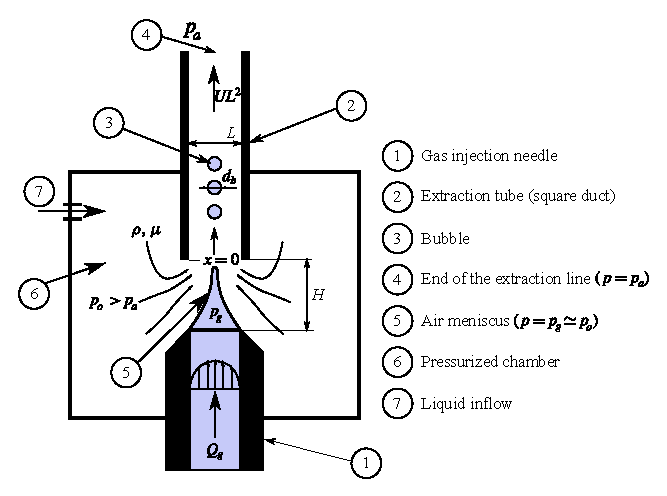
\includegraphics[scale=1]{introduccion/figuras/esquemaCSW.eps}
\caption{Esquema del dispositivo empleado en~\cite{Evangelio2015b} para la producción de microburbujas con la técnica de Confined Selective Withdrawal. Imagen adaptada de~\cite{Evangelio2015b}}
\LABFIG{esquemaCSW}
\end{figure}

 En la \FIG{esquemaCSW} se describe esquemáticamente el funcionamiento de este dispositivo. El dispositivo consiste en cámara presurizada a $p_{0}$ con un líquido, de densidad $\rho$ y de viscosidad $\mu$, que se suministra desde el exterior y que descarga a $p_{a} < p_{0}$ a través de una salida a través de un capilar (en este caso de sección cuadrada) de dimensiones características $L = 1\,\mathrm{mm}$. El capilar se encuentra perfectamente alineado con una aguja donde se inyecta el gas con caudal $Q_{g}$ y que se encuentra a una distancia $H$ del capilar. Como puede observarse en la \FIG{fenomenologia}, para velocidades del líquido en el capilar inferiores a una $U < U^{*}$, el menisco emite burbujas de forma pulsante y de diferentes diámetros~\cite{Evangelio2015b}. Sin embargo, por encima de esta velocidad, se puede observar que el menisco de aire se mantiene estable para una regíon $x \leq x_{s}$, lo que propicia la aparición de un régimen de producción de burbujas monodispersas; la condición de equilibrio de la que resulta $x_{s}$ será discutida más adelante. Finalmente, en la \FIG{produccionEstable} se muestra como, para valores de $U > U^{*}$, aguas abajo de la zona estacionaria ($x \leq x_{s}$), se produce un cilindro de gas de diámetro $d_{g}$ y longitud $\ell$ que, finalmente, culmina con la producción de una nueva burbuja; una vez la burbuja es emitida y transportada a la velocidad del líquido, se inicia nuevamente el proceso de formación de otra burbuja a través del mecanismo descrito. 
 
\begin{figure}[hbtp!]
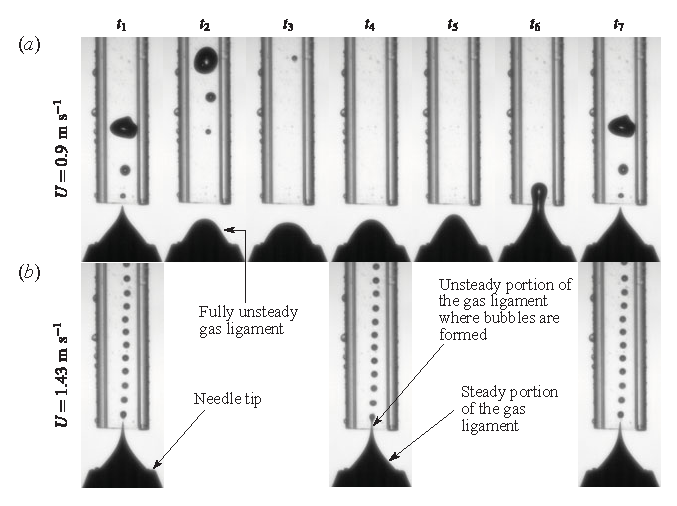
\includegraphics[scale=1]{introduccion/figuras/fenomenologia.eps}
\caption{Diferentes regímenes de burbujeo en función de la velocidad $U$ a la que el líquido circula a través del capilar. En (a) se visualiza el caso en que $U < U^{*}$, por lo que no se tiene un régimen de burbujeo constante, mientras que en (b), $U > U^{*}$, se consigue alcanzar un régimen de producción de burbujas monodispersas. Imágenes adaptadas de~\cite{Evangelio2015b}.}
\LABFIG{fenomenologia}
\end{figure}

Aunque en~\cite{Evangelio2015b} se analiza tanto el caso viscoso como el no viscoso, en esta sección nos centraremos únicamente en los casos $Re \gg 1$, ya que será el caso de interés para el dispositivo que aquí se describe. Antes de comenzar el análisis, conviene notar que la presión del gas, $p_{g}$, que además se considera constante a lo largo del mismo según la hipótesis ya comentada en la \SEC{fundamentos}, debe de encontrarse en equilibrio con la del líquido a la salida de la aguja, donde la velocidad del líquido es casi nula, por lo que puede suponerse que $p_{g} \simeq p_{0}$. Así, para obtener un menisco de aire estable en la región $x \leq x_{s}$, la diferencia de presiones $p_{0} - p\left(x\right)$ debe estar en equilibrio con la presión capilar. En efecto, considerando que el hilo gaseoso tenga un diámetro $d_{g}$, llamando $U_{0}$ a la velocidad en el centro del tubo capilar, y teniendo en cuenta el cumplimiento de la ecuación de continuidad

\begin{equation}
Q_{g} = \dfrac{\pi d_{g}^{2}}{4}U_{0} \Rightarrow d_{g} \sim \left(\dfrac{Q_{g}}{U_{0}}\right)^{1/2}
\LABEQ{continuidadLigamento}, 
\end{equation}

se tiene que 

\begin{equation}
p_{0} - p\left(x_{s}\right) = \dfrac{2\sigma}{d_{g}} \simeq \dfrac{2\sigma}{\left(Q_{g}/U_{0}\right)^{1/2}}
\LABEQ{equilibrioLigamento}
\end{equation}

lo que proporciona la condición de equilibrio para que exista un menisco de aire estacionario en $x \leq x_{s}$. Tanto en \eqref{eq:contiuidadLigamento} como en \eqref{equilibrioLigamento}, la expresión de $U_{0}$ vendrá determinada por el tipo de flujo que exista en el capilar, lo que para el caso en el que $Re \gg 1$ y teniendo en cuenta los resultados de las simulaciones
\footnote{En~\cite{Evangelio2015b} se realiza una simulación del dominio considerando este como axilsimétrico y sin simular la fase gaseosa, lo que suele realizarse generalmente cuando se desea estudiar la estabilidad de chorros, descomponiendo el campo de presiones como suma de la solución básica más una perturbación (véase como ejemplo~\cite{Gordillo2014a}. En~\cite{Evangelio2015b}, sin embargo, se realiza la hipótesis, verificada \textit{a posteriori}, de que la presencia de las burbujas no perturba el campo de presiones del líquido.} realizadas en~\cite{Evangelio2015b} constituye un perfil uniforme de velocidad; efectivamente, este hecho queda representado por el valor del coeficiente de presión adimensional $\xi = \left(p_{0} - p\left(x\right)\right)/\left(1/2 \rho U^{2}\right) \simeq 1$ en $x = 0$. Así, dado que $p_{0} - p\left(x_{s}\right) \sim 1/2\rho U^{2}$ para $Re \gg 1$ y teniendo en cuenta que la formación de burbujas tnedrá lugar si $p_{0}-p\left(x\right) > \dfrac{2\sigma}{d_{g}}$, la formación de burbujas monodispersas será posible si 

\begin{equation}
\beta = \dfrac{\rho U^{2} L}{4\sigma}q^{1/2} \gtrsim 1 \qquad \mathrm{con} q = \dfrac{Q_{g}}{UL^{2}}
\LABEQ{beta}
\end{equation}

donde $\beta$ en la \EQ{beta} constituye un parámetro similar al número de Webber, $We = \rho U^{2}L^{2}/\sigma$; la validez de \eqref{eq:beta} queda mostrada en~\cite{Evangelio2015b}.

\begin{figure}[hbtp!]
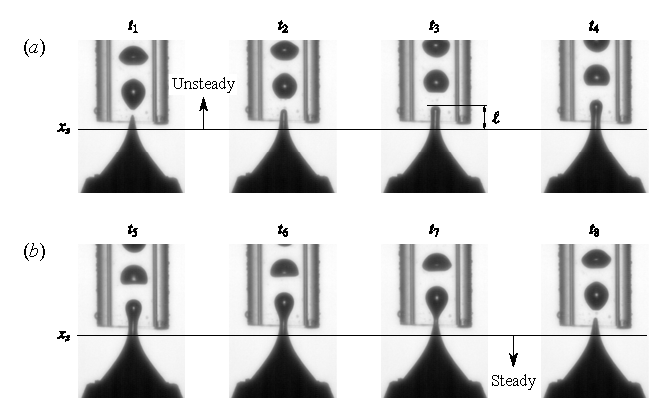
\includegraphics[scale=1]{introduccion/figuras/produccionEstable.eps}
\caption{Secuencia de producción de burbujas a partir de un menisco de aire estable para la región $x \leq x_{s}$. Como se aprecia en la figura, aguas abajo de $x_{s}$, se emite un cilindro de gas de diámetro $\sim d_{g}$ que se extiende una longitud $\ell$. Imagen tomada de~\cite{Evangelio2015b}.}
\LABFIG{produccionEstable}
\end{figure}


Una vez se han descrito las condiciones neesarias para la producción monodispersa de burbujas y se conocen las condiciones de equilibrio estacionario del menisco de aire, se está en condición de describir el resto del proceso de formación, así como las expresiones de los diámetros y frecuencias de producción de las burbujas obtenidas. Una vez que las burbujas se desprenden del ligamento de gas en $Lx \approx Lx_{s} + \ell$, la diferencia de presión $\Delta p = p_{0} - p\left(x\right) -2\sigma/d_{g} > 0$, induce velocidades radiales sobre el ligamento de gas que provoca el inicio del proceso de formación de una nueva burbuja. Dado que durante los instantes posteriores a la eyección de una nueva burbuja el diámetro del cilindro apenas varía, es posible escribir

\begin{equation}
\begin{split}
&\Delta p = p_{0} - p\left(x\right) - 2\sigma/d_{g} = p_{0} - p\left(x_{s}\right) - 2\sigma/d_{g} + p\left(x_{s}\right) - p\left(x\right) \approx \\
& \approx - \dfrac{\mathrm{d}p}{\mathrm{d} x}\left(x_{s}\right)\left(x-x_{s}\right) \approx \dfrac{\mathrm{d}\left(p_{0}-p\right)}{\mathrm{d}x}\left(x_{s}\right)\dfrac{\ell}{L}
\end{split}
\LABEQ{gradPress}
\end{equation}

donde se ha tenido en cuenta la \EQ{equilibrioLigamento} y se ha realizado un desarrollo en serie de Taylor de primer orden de la presión en torno al punto $x = x_{s}$. De este modo, y tal y como se detalla en~\cite{Evangelio2015b}, la \EQ{gradPress} muestra como el proceso de formación de burbujas está gobernado por el gradiente de presión local en el punto $x = x_{s}$, por lo que, como ya se ha comentado previamente, el gradiente de presión local posee un papel absolutamente análogo al que tiene la gravedad en la formación de una burbuja en una piscina en reposo. Por lo tanto, siguiendo el procedimiento que se siguió en la \SEC{fundamentos}, si se sustituye la \EQ{gradPress}, particularizada para el caso $Re \gg 1$, en la ecuación de Rayleigh-Plesset (\EQ{rayleighPlesset}), se tendrá que 

\begin{equation}
\rho R_{b}\ddot{R}_{b} \propto \dfrac{\mathrm{d}\left(p_{0} - p\right)}{\mathrm{d}x}\left(x_{s}\right)\dfrac{\ell}{L}\propto \dfrac{\ell}{2L}\rho U^{2} P_{s}
\end{equation}

siendo $P_{s} = \dot{\xi}\left(x_{s}\right)$. La ecuación anterior junto con la ecuación de continuidad~\eqref{eq:continuidad}, reescrita aquí por conveniencia

\begin{equation}
Q_{g} = \dfrac{\pi}{6}d_{b}^{3} f_{b}
\end{equation}

permiten obtener las frecuencias de producción,

\begin{equation}
\rho \dfrac{P_{s}}{2}\dfrac{U^{2}}{L}\ell \propto \rho R_{b} \ddot{R}_{b} \sim \rho d_{b}^{2}f_{b}^{2} \Rightarrow f_{b} \propto \dfrac{U\sqrt{P_{s}/2}}{\sqrt{L d_{b}}}\sqrt{\dfrac{\ell}{d_{b}}}
\LABEQ{freqGradPres}
\end{equation}

y, finalmente, tomando $\ell \propto d_{b}$ empleando la analogía al caso de formación de burbujas en una piscina en reposo~\cite{Evangelio2015b}, la expresión final de la frecuencia y los diámetros de las burbujas. 

\begin{equation}
f_{b} \propto \dfrac{U\sqrt{P_{s}/2}}{\sqrt{L d_{b}}} \quad \mathrm{y} \quad \dfrac{d_{b}}{L} \propto \left(\dfrac{Q_{g}}{U\sqrt{P_{s}/2}L^{2}}\right)^{2/5}
\end{equation}

El proceso seguido para la obtención de las ecuaciones~\eqref{eq:freqGradPres} y \eqref{dbGradPres} es completamente análogo al descrito en la \SEC{fundamentos} con el gradiente de presión local ejerciendo el papel de la gravedad y con la diferencia que $\rho U^{2}/L \gg \rho g $, lo que atendiendo a las ecuaciones de arriba, se traduce en un aumento de la frecuencia y una disminución de los diámetros obtenidos. Este hecho hace pensar que, si el proceso de formación descrito está controlado por el gradiente de presión local en $x_{s}$, nada impide pensar en dispositivos generadores de burbujas donde los gradientes favorables de presión puedan obtenerse con geometrías tan diversas como diferentes a la descrita en~\cite{Evangelio2015b}.


\section{Analogía Aerodinámica}\LABSEC{aerodynamics}

Al final de La \SEC{gradPres}, basándose en las ideas de~\cite{Evangelio2015b}, se dejó entrever la posibilidad de obtener gradientes favorables de presión similares a los encontrados en dispositivos de Confned Selective Withdrawal o Flow-Focussing pero con otras geometrías completamente diferentes. La motivación en la exploración de otras geometrías es doble: dispositivos con tamaños alejados de la escala de la microfluídica permitirían no sólo una fabricación y operación más sencilla sino también aumentar notablemente las frecuencias de producción de las burbujas. Así, un ejemplo cotidiano de geometrías donde se producen fuertes gradientes favorables de presión lo constituyen los perfiles aerodinámicos empleados como sección transversal en las alas de los aviones. Dado que la única premisa que, \textit{a priori}, debe cumplir una geometría alternativa a las empleadas actualmente sería conseguir gradientes de presión comparables a los creados en los dispositivos microfluídicos, ¿qué impide pensar que se pueda emplear un ala para producir masivamente microburbujas monodispersas?

Conviene antes de seguir, no obstante, esbozar algunas ideas básicas en aerodinámica que permitirán comprender mejor la posibilidad de emplear un ala como dispositivo generador de burbujas. La Aerodinámica es la parte de la Mecánica de Fluidos que se encarga del estudio del movimiento de gases (generalmente aire) alrededor de un cuerpo. Teniendo en cuenta las propiedades del aire (densidad $\rho_{g} \sim \mathcal{O}(1\,\mathrm{kg/m^{3}})$ y viscosidad $\mu \sim \mathcal{O}(10^{-5}\,\mathrm{Pa \cdot s})$ a $T = 20^{\circ}$) y las velocidades características de un cuerpo que se mueve en él (tómese como ejemplo un coche circulando a $V = 30\,\mathrm{m/s} $ o el ala de un avión a $V = 100\, \mathrm{m/s}$) se tiene que los números de Reynolds característicos del flujo de aire alrededor de un objeto con dimensiones características $L = 1\,\mathrm{m}$ serán $Re = \rho V L / \mu  \sim \mathcal{O}\left(10^{6}\right)$. Bajo estas condiciones los efectos viscosos pueden ser despreciados en la mayor parte del dominio del problema salvo en una delgada región adyacente a la superficie del cuerpo (capa límite), donde la viscosidad impone la condición de contorno de velocidad relativa nula para el fluido con respecto al sólido y donde, por lo tanto, los efectos de inercia y los viscosos son del mismo orden ($Re \approx 1$); el espesor de esta capa puede ser estimado como $\delta_{L} \sim L Re^{-1/2}$, por lo que para el caso del ala de un avión ($L \sim 1\,\mathrm{m}$) esta capa tiene un espesor de apróximadamente 1\,mm. Sin embargo, la importancia de esta delgada capa en la estabilidad del flujo alrededor del cuerpo es capital, ya que si sus efectos no estuvieran confinados a la mencionada región la hipótesis de viscosidad despreciable en el resto del dominio no sería asumible. En efecto, si la corriente experimenta un gradiente adverso de presión (como el que experimenta un fluido cuando circula a través de un canal que se ensancha o el que pueda existir en una esfera aguas abajo del punto más alto de la misma), las velocidades cerca de la pared del sólido son tan cercanas a cero que puede producirse una recirculación del fluido, lo que provocaría el desprendimiento de la capa límite. Para que esto no se produzca, se puede reducir el gradiente desfavorable de presión extediendo la longitud del cuerpo aguas abajo del punto de mínima presión, lo que para el caso de un sólido en el seno del aire significaría emplear cuerpos fuselados (cuerpos con longitud transversal característica mucho menor que la longitudinal) en lugar de cuerpos romos (como sería por ejemplo una esfera). Además, para que la corriente no se desprenda, el ángulo con el que incide la corriente con respecto a línea media longitudinal del sólido, no debe ser muy elevado, ya que de lo contrario el desprendimiento también tendrá lugar. 